\documentclass{report}
%%%%%%%%%%%%%%%%%%%%%%%%%%%%%%%%%
% PACKAGE IMPORTS
%%%%%%%%%%%%%%%%%%%%%%%%%%%%%%%%%


% Codificación y tipografía básica (se cargan aquí para orden correcto)
\usepackage[utf8]{inputenc}
\usepackage[T1]{fontenc}
\usepackage{lmodern}
% Idioma español para nombres de elementos flotantes (Figura, Tabla, etc.)
\usepackage[spanish]{babel}
% Asegurar nombre de tablas en español
\addto\captionsspanish{\renewcommand{\tablename}{Tabla}}


\usepackage[tmargin=2cm,rmargin=1in,lmargin=1in,margin=0.85in,bmargin=2cm,footskip=.2in]{geometry}
\usepackage{amsmath,amsfonts,amsthm,amssymb,mathtools}
\usepackage[varbb]{newpxmath}
\usepackage{xfrac}
\usepackage[makeroom]{cancel}
\usepackage{mathtools}
\usepackage{bookmark}
\usepackage{enumitem}
\usepackage{hyperref,theoremref}
\hypersetup{
	pdftitle={Assignment},
	colorlinks=true, linkcolor=gray,citecolor=blue,
	bookmarksnumbered=true,
	bookmarksopen=true
}
\usepackage[most,many,breakable]{tcolorbox}
\usepackage{xcolor}
\usepackage{varwidth}
\usepackage{varwidth}
\usepackage{etoolbox}
%\usepackage{authblk}
\usepackage{nameref}
\usepackage{multicol,array}
\usepackage{tikz-cd}
\usepackage[ruled,vlined,linesnumbered]{algorithm2e}
\usepackage{comment} % enables the use of multi-line comments (\ifx \fi) 
\usepackage{import}
\usepackage{xifthen}
\usepackage{pdfpages}
\usepackage{transparent}

\newcommand\mycommfont[1]{\footnotesize\ttfamily\textcolor{blue}{#1}}
\SetCommentSty{mycommfont}
\newcommand{\incfig}[1]{%
    \def\svgwidth{\columnwidth}
    \import{./figures/}{#1.pdf_tex}
}

\usepackage{tikzsymbols}
\renewcommand\qedsymbol{$\Laughey$}


%\usepackage{import}
%\usepackage{xifthen}
%\usepackage{pdfpages}
%\usepackage{transparent}


%%%%%%%%%%%%%%%%%%%%%%%%%%%%%%
% SELF MADE COLORS
%%%%%%%%%%%%%%%%%%%%%%%%%%%%%%



\definecolor{myg}{RGB}{56, 140, 70}
\definecolor{myb}{RGB}{45, 111, 177}
\definecolor{myr}{RGB}{199, 68, 64}
\definecolor{mytheorembg}{HTML}{F2F2F9}
\definecolor{mytheoremfr}{HTML}{00007B}
\definecolor{mylenmabg}{HTML}{FFFAF8}
\definecolor{mylenmafr}{HTML}{983b0f}
\definecolor{mypropbg}{HTML}{f2fbfc}
\definecolor{mypropfr}{HTML}{191971}
\definecolor{myexamplebg}{HTML}{F2FBF8}
\definecolor{myexamplefr}{HTML}{88D6D1}
\definecolor{myexampleti}{HTML}{2A7F7F}
\definecolor{mydefinitbg}{HTML}{E5E5FF}
\definecolor{mydefinitfr}{HTML}{3F3FA3}
\definecolor{notesgreen}{RGB}{0,162,0}
\definecolor{myp}{RGB}{197, 92, 212}
\definecolor{mygr}{HTML}{2C3338}
\definecolor{myred}{RGB}{127,0,0}
\definecolor{myyellow}{RGB}{169,121,69}
\definecolor{myexercisebg}{HTML}{F2FBF8}
\definecolor{myexercisefg}{HTML}{88D6D1}


%%%%%%%%%%%%%%%%%%%%%%%%%%%%
% TCOLORBOX SETUPS
%%%%%%%%%%%%%%%%%%%%%%%%%%%%

\setlength{\parindent}{1cm}
%================================
% THEOREM BOX
%================================

\tcbuselibrary{theorems,skins,hooks}
\newtcbtheorem[number within=section]{Theorem}{Theorem}
{%
	enhanced,
	breakable,
	colback = mytheorembg,
	frame hidden,
	boxrule = 0sp,
	borderline west = {2pt}{0pt}{mytheoremfr},
	sharp corners,
	detach title,
	before upper = \tcbtitle\par\smallskip,
	coltitle = mytheoremfr,
	fonttitle = \bfseries\sffamily,
	description font = \mdseries,
	separator sign none,
	segmentation style={solid, mytheoremfr},
}
{th}

\tcbuselibrary{theorems,skins,hooks}
\newtcbtheorem[number within=chapter]{theorem}{Theorem}
{%
	enhanced,
	breakable,
	colback = mytheorembg,
	frame hidden,
	boxrule = 0sp,
	borderline west = {2pt}{0pt}{mytheoremfr},
	sharp corners,
	detach title,
	before upper = \tcbtitle\par\smallskip,
	coltitle = mytheoremfr,
	fonttitle = \bfseries\sffamily,
	description font = \mdseries,
	separator sign none,
	segmentation style={solid, mytheoremfr},
}
{th}


\tcbuselibrary{theorems,skins,hooks}
\newtcolorbox{Theoremcon}
{%
	enhanced
	,breakable
	,colback = mytheorembg
	,frame hidden
	,boxrule = 0sp
	,borderline west = {2pt}{0pt}{mytheoremfr}
	,sharp corners
	,description font = \mdseries
	,separator sign none
}

%================================
% Corollery
%================================
\tcbuselibrary{theorems,skins,hooks}
\newtcbtheorem[number within=section]{Corollary}{Corollary}
{%
	enhanced
	,breakable
	,colback = myp!10
	,frame hidden
	,boxrule = 0sp
	,borderline west = {2pt}{0pt}{myp!85!black}
	,sharp corners
	,detach title
	,before upper = \tcbtitle\par\smallskip
	,coltitle = myp!85!black
	,fonttitle = \bfseries\sffamily
	,description font = \mdseries
	,separator sign none
	,segmentation style={solid, myp!85!black}
}
{th}
\tcbuselibrary{theorems,skins,hooks}
\newtcbtheorem[number within=chapter]{corollary}{Corollary}
{%
	enhanced
	,breakable
	,colback = myp!10
	,frame hidden
	,boxrule = 0sp
	,borderline west = {2pt}{0pt}{myp!85!black}
	,sharp corners
	,detach title
	,before upper = \tcbtitle\par\smallskip
	,coltitle = myp!85!black
	,fonttitle = \bfseries\sffamily
	,description font = \mdseries
	,separator sign none
	,segmentation style={solid, myp!85!black}
}
{th}


%================================
% LENMA
%================================

\tcbuselibrary{theorems,skins,hooks}
\newtcbtheorem[number within=section]{Lenma}{Lenma}
{%
	enhanced,
	breakable,
	colback = mylenmabg,
	frame hidden,
	boxrule = 0sp,
	borderline west = {2pt}{0pt}{mylenmafr},
	sharp corners,
	detach title,
	before upper = \tcbtitle\par\smallskip,
	coltitle = mylenmafr,
	fonttitle = \bfseries\sffamily,
	description font = \mdseries,
	separator sign none,
	segmentation style={solid, mylenmafr},
}
{th}

\tcbuselibrary{theorems,skins,hooks}
\newtcbtheorem[number within=chapter]{lenma}{Lenma}
{%
	enhanced,
	breakable,
	colback = mylenmabg,
	frame hidden,
	boxrule = 0sp,
	borderline west = {2pt}{0pt}{mylenmafr},
	sharp corners,
	detach title,
	before upper = \tcbtitle\par\smallskip,
	coltitle = mylenmafr,
	fonttitle = \bfseries\sffamily,
	description font = \mdseries,
	separator sign none,
	segmentation style={solid, mylenmafr},
}
{th}


%================================
% PROPOSITION
%================================

\tcbuselibrary{theorems,skins,hooks}
\newtcbtheorem[number within=section]{Prop}{Proposition}
{%
	enhanced,
	breakable,
	colback = mypropbg,
	frame hidden,
	boxrule = 0sp,
	borderline west = {2pt}{0pt}{mypropfr},
	sharp corners,
	detach title,
	before upper = \tcbtitle\par\smallskip,
	coltitle = mypropfr,
	fonttitle = \bfseries\sffamily,
	description font = \mdseries,
	separator sign none,
	segmentation style={solid, mypropfr},
}
{th}

\tcbuselibrary{theorems,skins,hooks}
\newtcbtheorem[number within=chapter]{prop}{Proposition}
{%
	enhanced,
	breakable,
	colback = mypropbg,
	frame hidden,
	boxrule = 0sp,
	borderline west = {2pt}{0pt}{mypropfr},
	sharp corners,
	detach title,
	before upper = \tcbtitle\par\smallskip,
	coltitle = mypropfr,
	fonttitle = \bfseries\sffamily,
	description font = \mdseries,
	separator sign none,
	segmentation style={solid, mypropfr},
}
{th}


%================================
% CLAIM
%================================

\tcbuselibrary{theorems,skins,hooks}
\newtcbtheorem[number within=section]{claim}{Claim}
{%
	enhanced
	,breakable
	,colback = myg!10
	,frame hidden
	,boxrule = 0sp
	,borderline west = {2pt}{0pt}{myg}
	,sharp corners
	,detach title
	,before upper = \tcbtitle\par\smallskip
	,coltitle = myg!85!black
	,fonttitle = \bfseries\sffamily
	,description font = \mdseries
	,separator sign none
	,segmentation style={solid, myg!85!black}
}
{th}



%================================
% Exercise
%================================

\tcbuselibrary{theorems,skins,hooks}
\newtcbtheorem[number within=section]{Exercise}{Exercise}
{%
	enhanced,
	breakable,
	colback = myexercisebg,
	frame hidden,
	boxrule = 0sp,
	borderline west = {2pt}{0pt}{myexercisefg},
	sharp corners,
	detach title,
	before upper = \tcbtitle\par\smallskip,
	coltitle = myexercisefg,
	fonttitle = \bfseries\sffamily,
	description font = \mdseries,
	separator sign none,
	segmentation style={solid, myexercisefg},
}
{th}

\tcbuselibrary{theorems,skins,hooks}
\newtcbtheorem[number within=chapter]{exercise}{Exercise}
{%
	enhanced,
	breakable,
	colback = myexercisebg,
	frame hidden,
	boxrule = 0sp,
	borderline west = {2pt}{0pt}{myexercisefg},
	sharp corners,
	detach title,
	before upper = \tcbtitle\par\smallskip,
	coltitle = myexercisefg,
	fonttitle = \bfseries\sffamily,
	description font = \mdseries,
	separator sign none,
	segmentation style={solid, myexercisefg},
}
{th}

%================================
% EXAMPLE BOX
%================================

\newtcbtheorem[number within=section]{Example}{Example}
{%
	colback = myexamplebg
	,breakable
	,colframe = myexamplefr
	,coltitle = myexampleti
	,boxrule = 1pt
	,sharp corners
	,detach title
	,before upper=\tcbtitle\par\smallskip
	,fonttitle = \bfseries
	,description font = \mdseries
	,separator sign none
	,description delimiters parenthesis
}
{ex}

\newtcbtheorem[number within=chapter]{example}{Example}
{%
	colback = myexamplebg
	,breakable
	,colframe = myexamplefr
	,coltitle = myexampleti
	,boxrule = 1pt
	,sharp corners
	,detach title
	,before upper=\tcbtitle\par\smallskip
	,fonttitle = \bfseries
	,description font = \mdseries
	,separator sign none
	,description delimiters parenthesis
}
{ex}

%================================
% DEFINITION BOX
%================================

\newtcbtheorem[number within=section]{Definition}{Definition}{enhanced,
	before skip=2mm,after skip=2mm, colback=red!5,colframe=red!80!black,boxrule=0.5mm,
	attach boxed title to top left={xshift=1cm,yshift*=1mm-\tcboxedtitleheight}, varwidth boxed title*=-3cm,
	boxed title style={frame code={
					\path[fill=tcbcolback]
					([yshift=-1mm,xshift=-1mm]frame.north west)
					arc[start angle=0,end angle=180,radius=1mm]
					([yshift=-1mm,xshift=1mm]frame.north east)
					arc[start angle=180,end angle=0,radius=1mm];
					\path[left color=tcbcolback!60!black,right color=tcbcolback!60!black,
						middle color=tcbcolback!80!black]
					([xshift=-2mm]frame.north west) -- ([xshift=2mm]frame.north east)
					[rounded corners=1mm]-- ([xshift=1mm,yshift=-1mm]frame.north east)
					-- (frame.south east) -- (frame.south west)
					-- ([xshift=-1mm,yshift=-1mm]frame.north west)
					[sharp corners]-- cycle;
				},interior engine=empty,
		},
	fonttitle=\bfseries,
	title={#2},#1}{def}
\newtcbtheorem[number within=chapter]{definition}{Definition}{enhanced,
	before skip=2mm,after skip=2mm, colback=red!5,colframe=red!80!black,boxrule=0.5mm,
	attach boxed title to top left={xshift=1cm,yshift*=1mm-\tcboxedtitleheight}, varwidth boxed title*=-3cm,
	boxed title style={frame code={
					\path[fill=tcbcolback]
					([yshift=-1mm,xshift=-1mm]frame.north west)
					arc[start angle=0,end angle=180,radius=1mm]
					([yshift=-1mm,xshift=1mm]frame.north east)
					arc[start angle=180,end angle=0,radius=1mm];
					\path[left color=tcbcolback!60!black,right color=tcbcolback!60!black,
						middle color=tcbcolback!80!black]
					([xshift=-2mm]frame.north west) -- ([xshift=2mm]frame.north east)
					[rounded corners=1mm]-- ([xshift=1mm,yshift=-1mm]frame.north east)
					-- (frame.south east) -- (frame.south west)
					-- ([xshift=-1mm,yshift=-1mm]frame.north west)
					[sharp corners]-- cycle;
				},interior engine=empty,
		},
	fonttitle=\bfseries,
	title={#2},#1}{def}



%================================
% Solution BOX
%================================

\makeatletter
\newtcbtheorem{question}{Pregunta}{enhanced,
	breakable,
	colback=white,
	colframe=myb!80!black,
	attach boxed title to top left={yshift*=-\tcboxedtitleheight},
	fonttitle=\bfseries,
	title={#2},
	boxed title size=title,
	boxed title style={%
			sharp corners,
			rounded corners=northwest,
			colback=tcbcolframe,
			boxrule=0pt,
		},
	underlay boxed title={%
			\path[fill=tcbcolframe] (title.south west)--(title.south east)
			to[out=0, in=180] ([xshift=5mm]title.east)--
			(title.center-|frame.east)
			[rounded corners=\kvtcb@arc] |-
			(frame.north) -| cycle;
		},
	#1
}{def}
\makeatother

%================================
% SOLUTION BOX
%================================

\makeatletter
\newtcolorbox{solution}{enhanced,
	breakable,
	colback=white,
	colframe=myg!80!black,
	attach boxed title to top left={yshift*=-\tcboxedtitleheight},
	title=Solution,
	boxed title size=title,
	boxed title style={%
			sharp corners,
			rounded corners=northwest,
			colback=tcbcolframe,
			boxrule=0pt,
		},
	underlay boxed title={%
			\path[fill=tcbcolframe] (title.south west)--(title.south east)
			to[out=0, in=180] ([xshift=5mm]title.east)--
			(title.center-|frame.east)
			[rounded corners=\kvtcb@arc] |-
			(frame.north) -| cycle;
		},
}
\makeatother

%================================
% Question BOX
%================================

\makeatletter
\newtcbtheorem{qstion}{Pregunta}{enhanced,
	breakable,
	colback=white,
	colframe=mygr,
	attach boxed title to top left={yshift*=-\tcboxedtitleheight},
	fonttitle=\bfseries,
	title={#2},
	boxed title size=title,
	boxed title style={%
			sharp corners,
			rounded corners=northwest,
			colback=tcbcolframe,
			boxrule=0pt,
		},
	underlay boxed title={%
			\path[fill=tcbcolframe] (title.south west)--(title.south east)
			to[out=0, in=180] ([xshift=5mm]title.east)--
			(title.center-|frame.east)
			[rounded corners=\kvtcb@arc] |-
			(frame.north) -| cycle;
		},
	#1
}{def}
\makeatother

\newtcbtheorem[number within=chapter]{wconc}{Wrong Concept}{
	breakable,
	enhanced,
	colback=white,
	colframe=myr,
	arc=0pt,
	outer arc=0pt,
	fonttitle=\bfseries\sffamily\large,
	colbacktitle=myr,
	attach boxed title to top left={},
	boxed title style={
			enhanced,
			skin=enhancedfirst jigsaw,
			arc=3pt,
			bottom=0pt,
			interior style={fill=myr}
		},
	#1
}{def}



%================================
% NOTE BOX
%================================

\usetikzlibrary{arrows,calc,shadows.blur}
\tcbuselibrary{skins}
\newtcolorbox{note}[1][]{%
	enhanced jigsaw,
	colback=gray!20!white,%
	colframe=gray!80!black,
	size=small,
	boxrule=1pt,
	title=\textbf{Nota:-},
	halign title=flush center,
	coltitle=black,
	breakable,
	drop shadow=black!50!white,
	attach boxed title to top left={xshift=1cm,yshift=-\tcboxedtitleheight/2,yshifttext=-\tcboxedtitleheight/2},
	minipage boxed title=1.5cm,
	boxed title style={%
			colback=white,
			size=fbox,
			boxrule=1pt,
			boxsep=2pt,
			underlay={%
					\coordinate (dotA) at ($(interior.west) + (-0.5pt,0)$);
					\coordinate (dotB) at ($(interior.east) + (0.5pt,0)$);
					\begin{scope}
						\clip (interior.north west) rectangle ([xshift=3ex]interior.east);
						\filldraw [white, blur shadow={shadow opacity=60, shadow yshift=-.75ex}, rounded corners=2pt] (interior.north west) rectangle (interior.south east);
					\end{scope}
					\begin{scope}[gray!80!black]
						\fill (dotA) circle (2pt);
						\fill (dotB) circle (2pt);
					\end{scope}
				},
		},
	#1,
}

%%%%%%%%%%%%%%%%%%%%%%%%%%%%%%
% SELF MADE COMMANDS
%%%%%%%%%%%%%%%%%%%%%%%%%%%%%%


\newcommand{\thm}[2]{\begin{Theorem}{#1}{}#2\end{Theorem}}
\newcommand{\cor}[2]{\begin{Corollary}{#1}{}#2\end{Corollary}}
\newcommand{\mlenma}[2]{\begin{Lenma}{#1}{}#2\end{Lenma}}
\newcommand{\mprop}[2]{\begin{Prop}{#1}{}#2\end{Prop}}
\newcommand{\clm}[3]{\begin{claim}{#1}{#2}#3\end{claim}}
\newcommand{\wc}[2]{\begin{wconc}{#1}{}\setlength{\parindent}{1cm}#2\end{wconc}}
\newcommand{\thmcon}[1]{\begin{Theoremcon}{#1}\end{Theoremcon}}
\newcommand{\ex}[2]{\begin{Example}{#1}{}#2\end{Example}}
\newcommand{\dfn}[2]{\begin{Definition}[colbacktitle=red!75!black]{#1}{}#2\end{Definition}}
\newcommand{\dfnc}[2]{\begin{definition}[colbacktitle=red!75!black]{#1}{}#2\end{definition}}
\newcommand{\qs}[2]{\begin{question}{#1}{}#2\end{question}}
\newcommand{\pf}[2]{\begin{myproof}[#1]#2\end{myproof}}
\newcommand{\nt}[1]{\begin{note}#1\end{note}}

\newcommand*\circled[1]{\tikz[baseline=(char.base)]{
		\node[shape=circle,draw,inner sep=1pt] (char) {#1};}}
\newcommand\getcurrentref[1]{%
	\ifnumequal{\value{#1}}{0}
	{??}
	{\the\value{#1}}%
}
\newcommand{\getCurrentSectionNumber}{\getcurrentref{section}}
\newenvironment{myproof}[1][\proofname]{%
	\proof[\bfseries #1: ]%
}{\endproof}

\newcommand{\mclm}[2]{\begin{myclaim}[#1]#2\end{myclaim}}
\newenvironment{myclaim}[1][\claimname]{\proof[\bfseries #1: ]}{}

\newcounter{mylabelcounter}

\makeatletter
\newcommand{\setword}[2]{%
	\phantomsection
	#1\def\@currentlabel{\unexpanded{#1}}\label{#2}%
}
\makeatother




\tikzset{
	symbol/.style={
			draw=none,
			every to/.append style={
					edge node={node [sloped, allow upside down, auto=false]{$#1$}}}
		}
}


% deliminators
\DeclarePairedDelimiter{\abs}{\lvert}{\rvert}
\DeclarePairedDelimiter{\norm}{\lVert}{\rVert}

\DeclarePairedDelimiter{\ceil}{\lceil}{\rceil}
\DeclarePairedDelimiter{\floor}{\lfloor}{\rfloor}
\DeclarePairedDelimiter{\round}{\lfloor}{\rceil}

\newsavebox\diffdbox
\newcommand{\slantedromand}{{\mathpalette\makesl{d}}}
\newcommand{\makesl}[2]{%
\begingroup
\sbox{\diffdbox}{$\mathsurround=0pt#1\mathrm{#2}$}%
\pdfsave
\pdfsetmatrix{1 0 0.2 1}%
\rlap{\usebox{\diffdbox}}%
\pdfrestore
\hskip\wd\diffdbox
\endgroup
}
\newcommand{\dd}[1][]{\ensuremath{\mathop{}\!\ifstrempty{#1}{%
\slantedromand\@ifnextchar^{\hspace{0.2ex}}{\hspace{0.1ex}}}%
{\slantedromand\hspace{0.2ex}^{#1}}}}
\ProvideDocumentCommand\dv{o m g}{%
  \ensuremath{%
    \IfValueTF{#3}{%
      \IfNoValueTF{#1}{%
        \frac{\dd #2}{\dd #3}%
      }{%
        \frac{\dd^{#1} #2}{\dd #3^{#1}}%
      }%
    }{%
      \IfNoValueTF{#1}{%
        \frac{\dd}{\dd #2}%
      }{%
        \frac{\dd^{#1}}{\dd #2^{#1}}%
      }%
    }%
  }%
}
\providecommand*{\pdv}[3][]{\frac{\partial^{#1}#2}{\partial#3^{#1}}}
%  - others
\DeclareMathOperator{\Lap}{\mathcal{L}}
\DeclareMathOperator{\Var}{Var} % varience
\DeclareMathOperator{\Cov}{Cov} % covarience
\DeclareMathOperator{\E}{E} % expected

% Since the amsthm package isn't loaded

% I prefer the slanted \leq
\let\oldleq\leq % save them in case they're every wanted
\let\oldgeq\geq
\renewcommand{\leq}{\leqslant}
\renewcommand{\geq}{\geqslant}

% % redefine matrix env to allow for alignment, use r as default
% \renewcommand*\env@matrix[1][r]{\hskip -\arraycolsep
%     \let\@ifnextchar\new@ifnextchar
%     \array{*\c@MaxMatrixCols #1}}


%\usepackage{framed}
%\usepackage{titletoc}
%\usepackage{etoolbox}
%\usepackage{lmodern}


%\patchcmd{\tableofcontents}{\contentsname}{\sffamily\contentsname}{}{}

%\renewenvironment{leftbar}
%{\def\FrameCommand{\hspace{6em}%
%		{\color{myyellow}\vrule width 2pt depth 6pt}\hspace{1em}}%
%	\MakeFramed{\parshape 1 0cm \dimexpr\textwidth-6em\relax\FrameRestore}\vskip2pt%
%}
%{\endMakeFramed}

%\titlecontents{chapter}
%[0em]{\vspace*{2\baselineskip}}
%{\parbox{4.5em}{%
%		\hfill\Huge\sffamily\bfseries\color{myred}\thecontentspage}%
%	\vspace*{-2.3\baselineskip}\leftbar\textsc{\small\chaptername~\thecontentslabel}\\\sffamily}
%{}{\endleftbar}
%\titlecontents{section}
%[8.4em]
%{\sffamily\contentslabel{3em}}{}{}
%{\hspace{0.5em}\nobreak\itshape\color{myred}\contentspage}
%\titlecontents{subsection}
%[8.4em]
%{\sffamily\contentslabel{3em}}{}{}  
%{\hspace{0.5em}\nobreak\itshape\color{myred}\contentspage}



%%%%%%%%%%%%%%%%%%%%%%%%%%%%%%%%%%%%%%%%%%%
% TABLE OF CONTENTS
%%%%%%%%%%%%%%%%%%%%%%%%%%%%%%%%%%%%%%%%%%%

\usepackage{tikz}
\definecolor{doc}{RGB}{0,60,110}
\usepackage{titletoc}
\contentsmargin{0cm}
\titlecontents{chapter}[3.7pc]
{\addvspace{30pt}%
	\begin{tikzpicture}[remember picture, overlay]%
		\draw[fill=doc!60,draw=doc!60] (-7,-.1) rectangle (-0.9,.5);%
		\pgftext[left,x=-3.5cm,y=0.2cm]{\color{white}\Large\sc\bfseries Módulo\ \thecontentslabel};%
	\end{tikzpicture}\color{doc!60}\large\sc\bfseries}%
{}
{}
{\;\titlerule\;\large\sc\bfseries Page \thecontentspage
	\begin{tikzpicture}[remember picture, overlay]
		\draw[fill=doc!60,draw=doc!60] (2pt,0) rectangle (4,0.1pt);
	\end{tikzpicture}}%
\titlecontents{section}[3.7pc]
{\addvspace{2pt}}
{\contentslabel[\thecontentslabel]{2pc}}
{}
{\hfill\small \thecontentspage}
[]

\titlecontents*{subsection}[4.7pc] % Mayor indentación para subsecciones
{\addvspace{1pt}\small} % Espaciado más limpio
{\thecontentslabel\quad} % Mostrar número de subsección (1.1.1, 1.1.2)
{}
{\hfill\small\thecontentspage\\} % Alinear el número de página correctamente


\makeatletter
\renewcommand{\tableofcontents}{%
	\chapter*{%
	  \vspace*{-20\p@}%
	  \begin{tikzpicture}[remember picture, overlay]%
		  \pgftext[right,x=15cm,y=0.2cm]{\color{doc!60}\Huge\sc\bfseries \contentsname};%
		  \draw[fill=doc!60,draw=doc!60] (13.5,-.75) rectangle (20,1);%
		  \clip (13.4,-.75) rectangle (20,1);
		  \pgftext[right,x=15cm,y=0.2cm]{\color{white}\Huge\sc\bfseries \contentsname};%
	  \end{tikzpicture}}%
	\@starttoc{toc}}
\makeatother

 % revisar en preamble \setcounter{tocdepth}{3}
%From M275 "Topology" at SJSU
\newcommand{\id}{\mathrm{id}}
\newcommand{\taking}[1]{\xrightarrow{#1}}
\newcommand{\inv}{^{-1}}

%From M170 "Introduction to Graph Theory" at SJSU
\DeclareMathOperator{\diam}{diam}
\DeclareMathOperator{\ord}{ord}
\newcommand{\defeq}{\overset{\mathrm{def}}{=}}

%From the USAMO .tex files
\newcommand{\ts}{\textsuperscript}
\newcommand{\dg}{^\circ}
\newcommand{\ii}{\item}

% % From Math 55 and Math 145 at Harvard
% \newenvironment{subproof}[1][Proof]{%
% \begin{proof}[#1] \renewcommand{\qedsymbol}{$\blacksquare$}}%
% {\end{proof}}

\newcommand{\liff}{\leftrightarrow}
\newcommand{\lthen}{\rightarrow}
\newcommand{\opname}{\operatorname}
\newcommand{\surjto}{\twoheadrightarrow}
\newcommand{\injto}{\hookrightarrow}
\newcommand{\On}{\mathrm{On}} % ordinals
\DeclareMathOperator{\img}{im} % Image
\DeclareMathOperator{\Img}{Im} % Image
\DeclareMathOperator{\coker}{coker} % Cokernel
\DeclareMathOperator{\Coker}{Coker} % Cokernel
\DeclareMathOperator{\Ker}{Ker} % Kernel
\DeclareMathOperator{\rank}{rank}
\DeclareMathOperator{\Spec}{Spec} % spectrum
\DeclareMathOperator{\Tr}{Tr} % trace
\DeclareMathOperator{\pr}{pr} % projection
\DeclareMathOperator{\ext}{ext} % extension
\DeclareMathOperator{\pred}{pred} % predecessor
\DeclareMathOperator{\dom}{dom} % domain
\DeclareMathOperator{\ran}{ran} % range
\DeclareMathOperator{\Hom}{Hom} % homomorphism
\DeclareMathOperator{\Mor}{Mor} % morphisms
\DeclareMathOperator{\End}{End} % endomorphism

\newcommand{\eps}{\epsilon}
\newcommand{\veps}{\varepsilon}
\newcommand{\ol}{\overline}
\newcommand{\ul}{\underline}
\newcommand{\wt}{\widetilde}
\newcommand{\wh}{\widehat}
\newcommand{\vocab}[1]{\textbf{\color{blue} #1}}
\providecommand{\half}{\frac{1}{2}}
\newcommand{\dang}{\measuredangle} %% Directed angle
\newcommand{\ray}[1]{\overrightarrow{#1}}
\newcommand{\seg}[1]{\overline{#1}}
\newcommand{\arc}[1]{\wideparen{#1}}
\DeclareMathOperator{\cis}{cis}
\DeclareMathOperator*{\lcm}{lcm}
\DeclareMathOperator*{\argmin}{arg min}
\DeclareMathOperator*{\argmax}{arg max}
\newcommand{\cycsum}{\sum_{\mathrm{cyc}}}
\newcommand{\symsum}{\sum_{\mathrm{sym}}}
\newcommand{\cycprod}{\prod_{\mathrm{cyc}}}
\newcommand{\symprod}{\prod_{\mathrm{sym}}}
\newcommand{\Qed}{\begin{flushright}\qed\end{flushright}}
\newcommand{\parinn}{\setlength{\parindent}{1cm}}
\newcommand{\parinf}{\setlength{\parindent}{0cm}}
% \newcommand{\norm}{\|\cdot\|}
\newcommand{\inorm}{\norm_{\infty}}
\newcommand{\opensets}{\{V_{\alpha}\}_{\alpha\in I}}
\newcommand{\oset}{V_{\alpha}}
\newcommand{\opset}[1]{V_{\alpha_{#1}}}
\newcommand{\lub}{\text{lub}}
\newcommand{\del}[2]{\frac{\partial #1}{\partial #2}}
\newcommand{\Del}[3]{\frac{\partial^{#1} #2}{\partial^{#1} #3}}
\newcommand{\deld}[2]{\dfrac{\partial #1}{\partial #2}}
\newcommand{\Deld}[3]{\dfrac{\partial^{#1} #2}{\partial^{#1} #3}}
\newcommand{\lm}{\lambda}
\newcommand{\uin}{\mathbin{\rotatebox[origin=c]{90}{$\in$}}}
\newcommand{\usubset}{\mathbin{\rotatebox[origin=c]{90}{$\subset$}}}
\newcommand{\lt}{\left}
\newcommand{\rt}{\right}
\newcommand{\bs}[1]{\boldsymbol{#1}}
\newcommand{\exs}{\exists}
\newcommand{\st}{\strut}
\newcommand{\dps}[1]{\displaystyle{#1}}

\newcommand{\sol}{\setlength{\parindent}{0cm}\textbf{\textit{Solution:}}\setlength{\parindent}{1cm} }
\newcommand{\solve}[1]{\setlength{\parindent}{0cm}\textbf{\textit{Solución: }}\setlength{\parindent}{1cm}#1 \Qed}

% Things Lie
\newcommand{\kb}{\mathfrak b}
\newcommand{\kg}{\mathfrak g}
\newcommand{\kh}{\mathfrak h}
\newcommand{\kn}{\mathfrak n}
\newcommand{\ku}{\mathfrak u}
\newcommand{\kz}{\mathfrak z}
\DeclareMathOperator{\Ext}{Ext} % Ext functor
\DeclareMathOperator{\Tor}{Tor} % Tor functor
\newcommand{\gl}{\opname{\mathfrak{gl}}} % frak gl group
\renewcommand{\sl}{\opname{\mathfrak{sl}}} % frak sl group chktex 6

% More script letters etc.
\newcommand{\SA}{\mathcal A}
\newcommand{\SB}{\mathcal B}
\newcommand{\SC}{\mathcal C}
\newcommand{\SF}{\mathcal F}
\newcommand{\SG}{\mathcal G}
\newcommand{\SH}{\mathcal H}
\newcommand{\OO}{\mathcal O}

\newcommand{\SCA}{\mathscr A}
\newcommand{\SCB}{\mathscr B}
\newcommand{\SCC}{\mathscr C}
\newcommand{\SCD}{\mathscr D}
\newcommand{\SCE}{\mathscr E}
\newcommand{\SCF}{\mathscr F}
\newcommand{\SCG}{\mathscr G}
\newcommand{\SCH}{\mathscr H}

% Mathfrak primes
\newcommand{\km}{\mathfrak m}
\newcommand{\kp}{\mathfrak p}
\newcommand{\kq}{\mathfrak q}

% number sets
\newcommand{\RR}[1][]{\ensuremath{\ifstrempty{#1}{\mathbb{R}}{\mathbb{R}^{#1}}}}
\newcommand{\NN}[1][]{\ensuremath{\ifstrempty{#1}{\mathbb{N}}{\mathbb{N}^{#1}}}}
\newcommand{\ZZ}[1][]{\ensuremath{\ifstrempty{#1}{\mathbb{Z}}{\mathbb{Z}^{#1}}}}
\newcommand{\QQ}[1][]{\ensuremath{\ifstrempty{#1}{\mathbb{Q}}{\mathbb{Q}^{#1}}}}
\newcommand{\CC}[1][]{\ensuremath{\ifstrempty{#1}{\mathbb{C}}{\mathbb{C}^{#1}}}}
\newcommand{\PP}[1][]{\ensuremath{\ifstrempty{#1}{\mathbb{P}}{\mathbb{P}^{#1}}}}
\newcommand{\HH}[1][]{\ensuremath{\ifstrempty{#1}{\mathbb{H}}{\mathbb{H}^{#1}}}}
\newcommand{\FF}[1][]{\ensuremath{\ifstrempty{#1}{\mathbb{F}}{\mathbb{F}^{#1}}}}
% expected value
\newcommand{\EE}{\ensuremath{\mathbb{E}}}
\newcommand{\charin}{\text{ char }}
\DeclareMathOperator{\sign}{sign}
\DeclareMathOperator{\Aut}{Aut}
\DeclareMathOperator{\Inn}{Inn}
\DeclareMathOperator{\Syl}{Syl}
\DeclareMathOperator{\Gal}{Gal}
\DeclareMathOperator{\GL}{GL} % General linear group
\DeclareMathOperator{\SL}{SL} % Special linear group

%---------------------------------------
% BlackBoard Math Fonts :-
%---------------------------------------

%Captital Letters
\newcommand{\bbA}{\mathbb{A}}	\newcommand{\bbB}{\mathbb{B}}
\newcommand{\bbC}{\mathbb{C}}	\newcommand{\bbD}{\mathbb{D}}
\newcommand{\bbE}{\mathbb{E}}	\newcommand{\bbF}{\mathbb{F}}
\newcommand{\bbG}{\mathbb{G}}	\newcommand{\bbH}{\mathbb{H}}
\newcommand{\bbI}{\mathbb{I}}	\newcommand{\bbJ}{\mathbb{J}}
\newcommand{\bbK}{\mathbb{K}}	\newcommand{\bbL}{\mathbb{L}}
\newcommand{\bbM}{\mathbb{M}}	\newcommand{\bbN}{\mathbb{N}}
\newcommand{\bbO}{\mathbb{O}}	\newcommand{\bbP}{\mathbb{P}}
\newcommand{\bbQ}{\mathbb{Q}}	\newcommand{\bbR}{\mathbb{R}}
\newcommand{\bbS}{\mathbb{S}}	\newcommand{\bbT}{\mathbb{T}}
\newcommand{\bbU}{\mathbb{U}}	\newcommand{\bbV}{\mathbb{V}}
\newcommand{\bbW}{\mathbb{W}}	\newcommand{\bbX}{\mathbb{X}}
\newcommand{\bbY}{\mathbb{Y}}	\newcommand{\bbZ}{\mathbb{Z}}

%---------------------------------------
% MathCal Fonts :-
%---------------------------------------

%Captital Letters
\newcommand{\mcA}{\mathcal{A}}	\newcommand{\mcB}{\mathcal{B}}
\newcommand{\mcC}{\mathcal{C}}	\newcommand{\mcD}{\mathcal{D}}
\newcommand{\mcE}{\mathcal{E}}	\newcommand{\mcF}{\mathcal{F}}
\newcommand{\mcG}{\mathcal{G}}	\newcommand{\mcH}{\mathcal{H}}
\newcommand{\mcI}{\mathcal{I}}	\newcommand{\mcJ}{\mathcal{J}}
\newcommand{\mcK}{\mathcal{K}}	\newcommand{\mcL}{\mathcal{L}}
\newcommand{\mcM}{\mathcal{M}}	\newcommand{\mcN}{\mathcal{N}}
\newcommand{\mcO}{\mathcal{O}}	\newcommand{\mcP}{\mathcal{P}}
\newcommand{\mcQ}{\mathcal{Q}}	\newcommand{\mcR}{\mathcal{R}}
\newcommand{\mcS}{\mathcal{S}}	\newcommand{\mcT}{\mathcal{T}}
\newcommand{\mcU}{\mathcal{U}}	\newcommand{\mcV}{\mathcal{V}}
\newcommand{\mcW}{\mathcal{W}}	\newcommand{\mcX}{\mathcal{X}}
\newcommand{\mcY}{\mathcal{Y}}	\newcommand{\mcZ}{\mathcal{Z}}


%---------------------------------------
% Bold Math Fonts :-
%---------------------------------------

%Captital Letters
\newcommand{\bmA}{\boldsymbol{A}}	\newcommand{\bmB}{\boldsymbol{B}}
\newcommand{\bmC}{\boldsymbol{C}}	\newcommand{\bmD}{\boldsymbol{D}}
\newcommand{\bmE}{\boldsymbol{E}}	\newcommand{\bmF}{\boldsymbol{F}}
\newcommand{\bmG}{\boldsymbol{G}}	\newcommand{\bmH}{\boldsymbol{H}}
\newcommand{\bmI}{\boldsymbol{I}}	\newcommand{\bmJ}{\boldsymbol{J}}
\newcommand{\bmK}{\boldsymbol{K}}	\newcommand{\bmL}{\boldsymbol{L}}
\newcommand{\bmM}{\boldsymbol{M}}	\newcommand{\bmN}{\boldsymbol{N}}
\newcommand{\bmO}{\boldsymbol{O}}	\newcommand{\bmP}{\boldsymbol{P}}
\newcommand{\bmQ}{\boldsymbol{Q}}	\newcommand{\bmR}{\boldsymbol{R}}
\newcommand{\bmS}{\boldsymbol{S}}	\newcommand{\bmT}{\boldsymbol{T}}
\newcommand{\bmU}{\boldsymbol{U}}	\newcommand{\bmV}{\boldsymbol{V}}
\newcommand{\bmW}{\boldsymbol{W}}	\newcommand{\bmX}{\boldsymbol{X}}
\newcommand{\bmY}{\boldsymbol{Y}}	\newcommand{\bmZ}{\boldsymbol{Z}}
%Small Letters
\newcommand{\bma}{\boldsymbol{a}}	\newcommand{\bmb}{\boldsymbol{b}}
\newcommand{\bmc}{\boldsymbol{c}}	\newcommand{\bmd}{\boldsymbol{d}}
\newcommand{\bme}{\boldsymbol{e}}	\newcommand{\bmf}{\boldsymbol{f}}
\newcommand{\bmg}{\boldsymbol{g}}	\newcommand{\bmh}{\boldsymbol{h}}
\newcommand{\bmi}{\boldsymbol{i}}	\newcommand{\bmj}{\boldsymbol{j}}
\newcommand{\bmk}{\boldsymbol{k}}	\newcommand{\bml}{\boldsymbol{l}}
\newcommand{\bmm}{\boldsymbol{m}}	\newcommand{\bmn}{\boldsymbol{n}}
\newcommand{\bmo}{\boldsymbol{o}}	\newcommand{\bmp}{\boldsymbol{p}}
\newcommand{\bmq}{\boldsymbol{q}}	\newcommand{\bmr}{\boldsymbol{r}}
\newcommand{\bms}{\boldsymbol{s}}	\newcommand{\bmt}{\boldsymbol{t}}
\newcommand{\bmu}{\boldsymbol{u}}	\newcommand{\bmv}{\boldsymbol{v}}
\newcommand{\bmw}{\boldsymbol{w}}	\newcommand{\bmx}{\boldsymbol{x}}
\newcommand{\bmy}{\boldsymbol{y}}	\newcommand{\bmz}{\boldsymbol{z}}

%---------------------------------------
% Scr Math Fonts :-
%---------------------------------------

\newcommand{\sA}{{\mathscr{A}}}   \newcommand{\sB}{{\mathscr{B}}}
\newcommand{\sC}{{\mathscr{C}}}   \newcommand{\sD}{{\mathscr{D}}}
\newcommand{\sE}{{\mathscr{E}}}   \newcommand{\sF}{{\mathscr{F}}}
\newcommand{\sG}{{\mathscr{G}}}   \newcommand{\sH}{{\mathscr{H}}}
\newcommand{\sI}{{\mathscr{I}}}   \newcommand{\sJ}{{\mathscr{J}}}
\newcommand{\sK}{{\mathscr{K}}}   \newcommand{\sL}{{\mathscr{L}}}
\newcommand{\sM}{{\mathscr{M}}}   \newcommand{\sN}{{\mathscr{N}}}
\newcommand{\sO}{{\mathscr{O}}}   \newcommand{\sP}{{\mathscr{P}}}
\newcommand{\sQ}{{\mathscr{Q}}}   \newcommand{\sR}{{\mathscr{R}}}
\newcommand{\sS}{{\mathscr{S}}}   \newcommand{\sT}{{\mathscr{T}}}
\newcommand{\sU}{{\mathscr{U}}}   \newcommand{\sV}{{\mathscr{V}}}
\newcommand{\sW}{{\mathscr{W}}}   \newcommand{\sX}{{\mathscr{X}}}
\newcommand{\sY}{{\mathscr{Y}}}   \newcommand{\sZ}{{\mathscr{Z}}}


%---------------------------------------
% Math Fraktur Font
%---------------------------------------

%Captital Letters
\newcommand{\mfA}{\mathfrak{A}}	\newcommand{\mfB}{\mathfrak{B}}
\newcommand{\mfC}{\mathfrak{C}}	\newcommand{\mfD}{\mathfrak{D}}
\newcommand{\mfE}{\mathfrak{E}}	\newcommand{\mfF}{\mathfrak{F}}
\newcommand{\mfG}{\mathfrak{G}}	\newcommand{\mfH}{\mathfrak{H}}
\newcommand{\mfI}{\mathfrak{I}}	\newcommand{\mfJ}{\mathfrak{J}}
\newcommand{\mfK}{\mathfrak{K}}	\newcommand{\mfL}{\mathfrak{L}}
\newcommand{\mfM}{\mathfrak{M}}	\newcommand{\mfN}{\mathfrak{N}}
\newcommand{\mfO}{\mathfrak{O}}	\newcommand{\mfP}{\mathfrak{P}}
\newcommand{\mfQ}{\mathfrak{Q}}	\newcommand{\mfR}{\mathfrak{R}}
\newcommand{\mfS}{\mathfrak{S}}	\newcommand{\mfT}{\mathfrak{T}}
\newcommand{\mfU}{\mathfrak{U}}	\newcommand{\mfV}{\mathfrak{V}}
\newcommand{\mfW}{\mathfrak{W}}	\newcommand{\mfX}{\mathfrak{X}}
\newcommand{\mfY}{\mathfrak{Y}}	\newcommand{\mfZ}{\mathfrak{Z}}
%Small Letters
\newcommand{\mfa}{\mathfrak{a}}	\newcommand{\mfb}{\mathfrak{b}}
\newcommand{\mfc}{\mathfrak{c}}	\newcommand{\mfd}{\mathfrak{d}}
\newcommand{\mfe}{\mathfrak{e}}	\newcommand{\mff}{\mathfrak{f}}
\newcommand{\mfg}{\mathfrak{g}}	\newcommand{\mfh}{\mathfrak{h}}
\newcommand{\mfi}{\mathfrak{i}}	\newcommand{\mfj}{\mathfrak{j}}
\newcommand{\mfk}{\mathfrak{k}}	\newcommand{\mfl}{\mathfrak{l}}
\newcommand{\mfm}{\mathfrak{m}}	\newcommand{\mfn}{\mathfrak{n}}
\newcommand{\mfo}{\mathfrak{o}}	\newcommand{\mfp}{\mathfrak{p}}
\newcommand{\mfq}{\mathfrak{q}}	\newcommand{\mfr}{\mathfrak{r}}
\newcommand{\mfs}{\mathfrak{s}}	\newcommand{\mft}{\mathfrak{t}}
\newcommand{\mfu}{\mathfrak{u}}	\newcommand{\mfv}{\mathfrak{v}}
\newcommand{\mfw}{\mathfrak{w}}	\newcommand{\mfx}{\mathfrak{x}}
\newcommand{\mfy}{\mathfrak{y}}	\newcommand{\mfz}{\mathfrak{z}}

\usepackage[utf8]{inputenc}  % para PDFLaTeX
\usepackage[T1]{fontenc}
\usepackage{graphicx}
\usepackage{chemfig}
\usepackage{multicol}
\usepackage{booktabs}
\usepackage{siunitx}
\usepackage{cancel}
\usepackage{adjustbox}
\usepackage{pdflscape}  % permite páginas horizontales que se ven rotadas en el PDF
\usepackage[backend=biber, style=apa]{biblatex}
\usepackage{caption}
\usepackage[spanish]{babel}
\usepackage{lmodern}
\usepackage{multirow}
\usepackage{csquotes}
\addto\captionsspanish{
  \renewcommand{\contentsname}{Índice}
}

%% para mas adelante los modulos/capitulos deberian ir con \include{chapters/03-metodologia}

\graphicspath{{Doc/Fotos/}}
\addbibresource{Referencias.bib} % nombre de tu archivo .bib




\title{
    
\includegraphics[width=0.4\textwidth]{escudo.png}\\[2cm] % logo arriba
    {\Huge Materias Primas}\\[2em]
    {\Huge Obtención de Bioethanol a partir de huesos de aceituna}\\[2em]
}
\vspace{2em}
\author{\Large Pérez Hita, Christian  \\[1em] }
\vspace{1cm}
\date{07 de Enero de 2026}

\begin{document}
\setcounter{tocdepth}{3}
\maketitle
\newpage % or \cleardoublepage
% \pdfbookmark[<level>]{<title>}{<dest>}
\pdfbookmark[section]{\contentsname}{contenidos}

\tableofcontents
\pagebreak
\chapter{}
\section{Introducción}
\begin{flushleft}
He decidido tratar este tema debido a que es un proceso realmente interesante. Además, tras hablarlo con el profesor Javier Ochando, considero que podría ser un posible tema de TFG para el próximo curso.

Actualmente, en este curso se está proponiendo el mismo tema, pero con otro enfoque: la obtención de bioetanol mediante vía química en lugar de enzimática. Por lo tanto, además de obtener bioetanol mediante este método, también se pueden obtener otros productos de valor añadido, como lignina, biogás, biofertilizantes o incluso sulfato de amonio.

Asimismo, se podría haber obtenido furfural al reducir parte de la producción de bioetanol; sin embargo, al tratarse de la primera etapa del trabajo, aún no se ha evaluado cuál de las dos opciones presenta una mayor viabilidad económica y ambiental.
\end{flushleft}
Para el pretratamiento de los huesos de aceituna me he basado principalmente en \cite{Padilla-Rascon2022} tal y como se puede ver en la siguiente imagen:

\begin{figure}[h!]
    \centering
    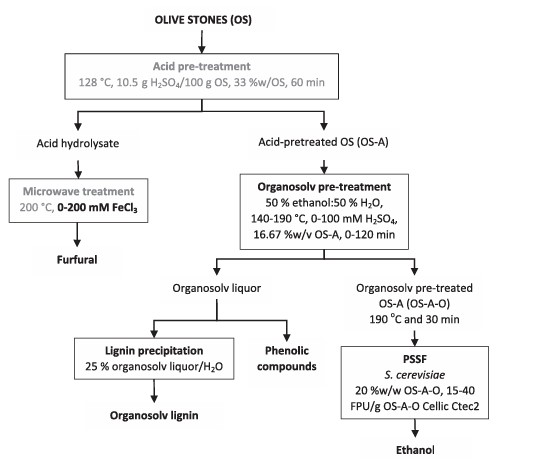
\includegraphics[width=0.55\textwidth]{Fotos/Pretratamiento.jpg}
    \caption{Esquema del pretratamiento de huesos de aceituna. Fuente:\cite{Padilla-Rascon2022}}
    \label{fig:pretratamiento}
\end{figure}


\chapter{}
\section{Justificación del producto seleccionado}
\begin{flushleft}
He decidido tratar este tema debido a que es realmente un proceso muy interesante ademas, tras hablarlo con el profesor Javier Ochando, para proponerlo como posible tema de TFG para el proximo curso.\\
Actualmente se esta proponiendo en este curso el mismo tema pero con otro enfoque, la obtención de bioethanol mediamente via química en lugar de enzimatica, por lo que aparte de obtener el bioethanol con este metodo se puede obtener otros productos de valor añadido como la lignina o el biogás biofertilizantes o el propio sulfato de amonio.\\
Tambien se podia haber obtenido furfural reduciendo parte de la generación de bioethanol pero al ser una primera etapa del trabajo no se ha evaluado cual de las dos opciones tiene una mayor viabilidad económica y ambiental.\\
\end{flushleft}
\vspace{1em}
Ademas recientemente se esta investigando mucho en la valorización de los residuos por ello he podido basarme en los siguientes articulos:
Propuesta de biorrefinería integral con PSSF y producción de biogás~\cite{Jafari-Gohargan2026}.

\medskip % Esto da un espacio vertical agradable entre párrafos

Estudio combinado de hidrólisis ácida y pretratamiento Organosolv~\cite{Padilla-Rascon2022}.

\medskip

Análisis de distintas estrategias para la obtención de bioetanol a partir de hueso de aceituna~\cite{Romero-Garca2022}.

\medskip

Evaluación del efecto del pretratamiento en el proceso de presacarificación y fermentación simultánea (PSSF)~\cite{AbuTayeh2026}.

\medskip

Estudio del proceso de detoxificación y fermentación de la fracción líquida rica en xilosa~\cite{TormosBelda2021}.

\chapter{}
\section{Diagrama de bloques}
\begin{figure}[h!]
    \centering
    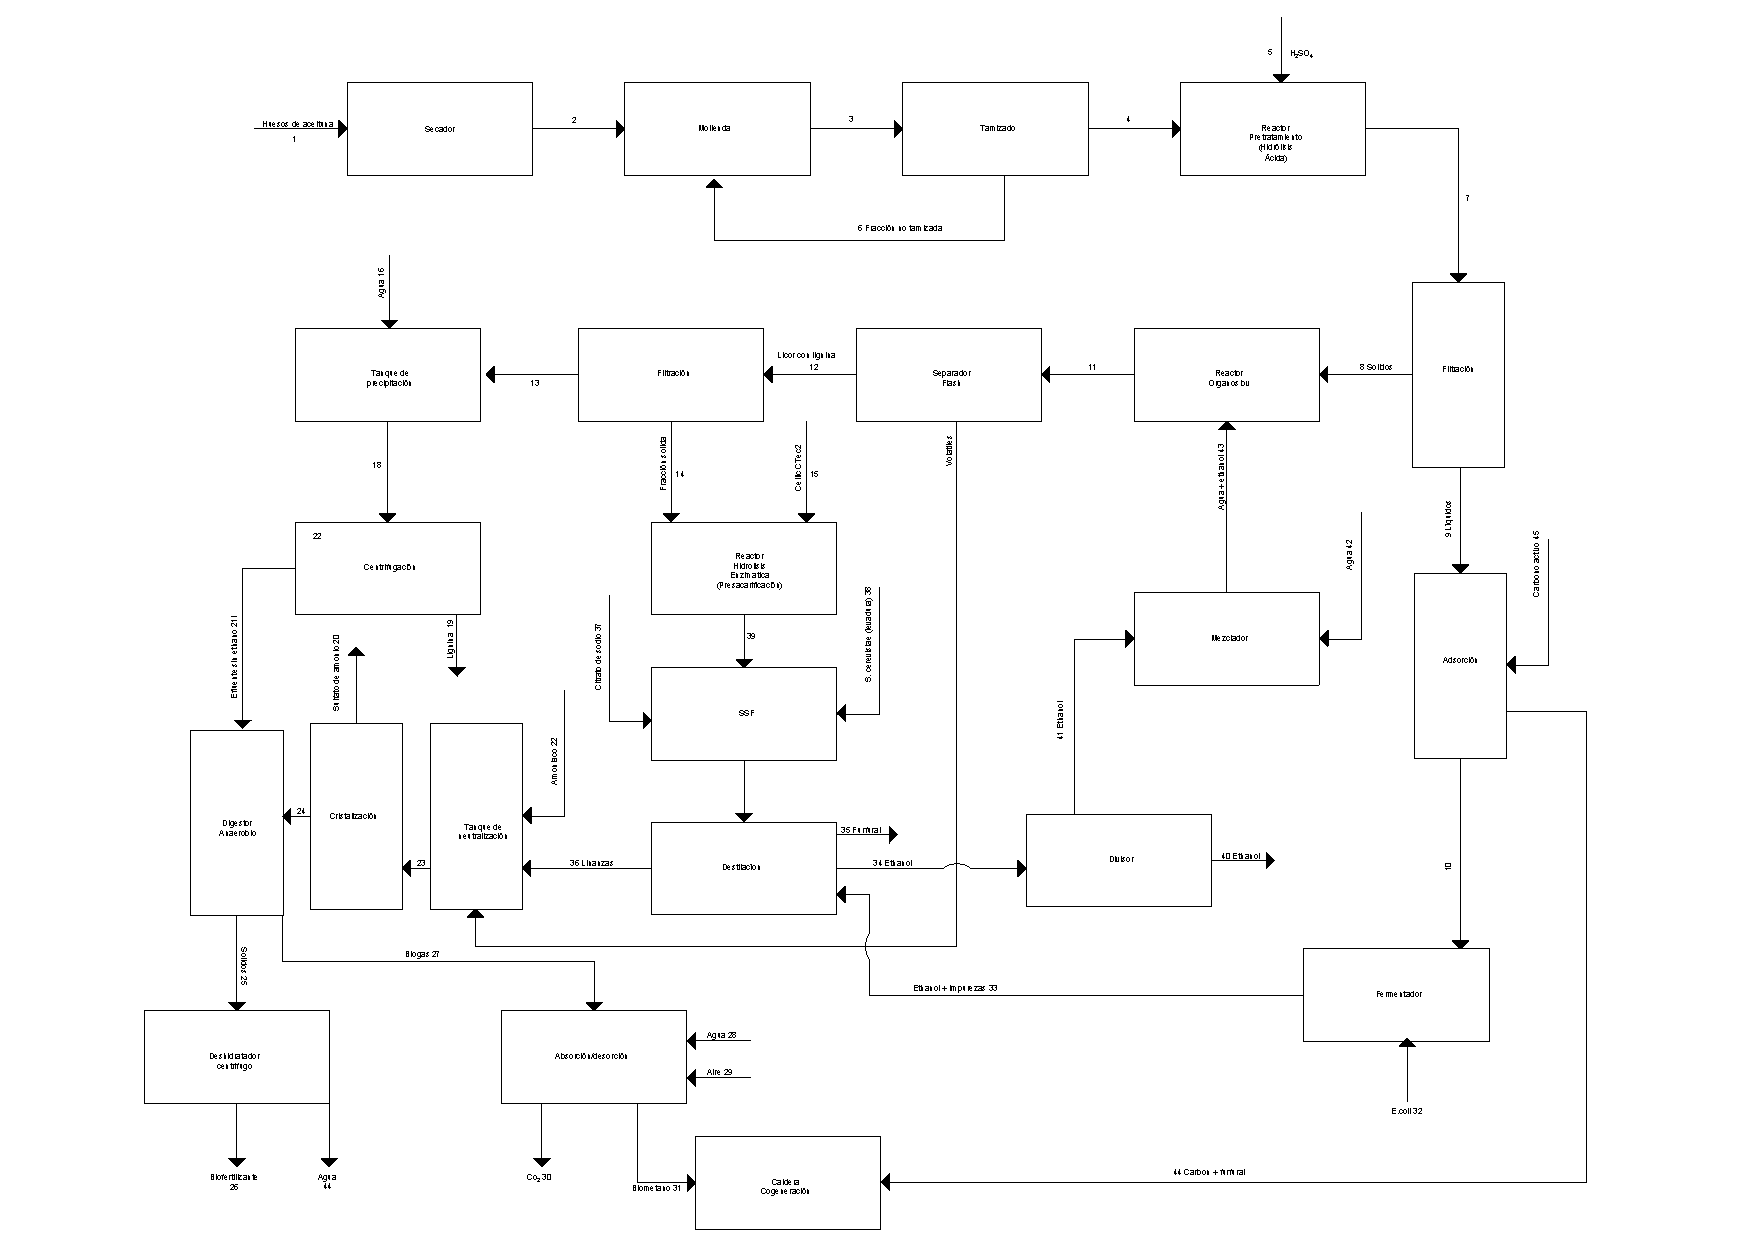
\includegraphics[width=0.95\textwidth]{Fotos/D-bloques.pdf}
    \caption{Esquema del proceso fuente: elaboración propia}
    \label{fig:proceso}
\end{figure}
\newpage

\section{Equipos necesarios}
Para los equipos necesarios en el proceso hay que destacar 3 lineas principales:
\begin{itemize}
    \item Linea principal de producción de bioetanol,(Fracción Sólida / Celulosa) Es la línea que procesa el sólido remanente tras el pretratamiento ácido inicial.
    \item Línea de Detoxificación (Fracción Líquida / Hemicelulosa) Es la línea que procesa el líquido que se separa al principio ( tras el prehidrolizado ácido).
    \item Línea de Valorización de Residuos (Biogás) Es la línea que trata los efluentes finales para cerrar el ciclo (Economía Circular).
\end{itemize}
Ademas para el transporte de la materia prima y productos a lo largo del proceso se necesitan equipos que se pueden ver en la siguiente tabla:

\begin{table}[h]
\centering
\begin{tabular}{|l|l|p{6cm}|}
\hline
\textbf{Tipo de Equipo} & \textbf{Ubicación en el Proceso} & \textbf{Función Específica} \\ \hline
\multirow{3}{*}{\textbf{Cinta Transportadora}} 
 & Recepción de Materia Prima & Traslado del hueso de aceituna desde el camión/patio de acopio hasta la tolva del molino . \\ \cline{2-3}
 & Alimentación Reactor 1 & Transporte del hueso molido y seco hacia la boca de entrada del reactor de pretratamiento ácido. \\ \cline{2-3}
 & Salida de Sólidos (Lignina) & Transporte de la lignina sólida precipitada y filtrada hacia la zona de secado o caldera. \\ \hline
\multirow{4}{*}{\textbf{Bomba Hidráulica}} 
 & Alimentación de Reactivos & Impulsión de agua, ácido sulfúrico diluido y etanol hacia los reactores de pretratamiento a alta presión. \\ \cline{2-3}
 & Transferencia entre Etapas & Movimiento de licores (hidrolizados) desde los filtros hacia las columnas de detoxificación y fermentadores. \\ \cline{2-3}
 & Alimentación a Destilación & Bombeo del "caldo" de fermentación (beer) hacia la primera columna de destilación . \\ \cline{2-3}
 & Gestión de Vinazas & Bombeo de los residuos líquidos del fondo de la destilación hacia el digestor anaerobio . \\ \hline
\multirow{3}{*}{\textbf{Compresor}} 
 & Unidad de Biogás (Upgrading) & Compresión del biogás a 10 bar antes de entrar a la columna de absorción con agua para separar el CO$_2$ . \\ \cline{2-3}
 & Almacenamiento de Gas & Compresión del biometano purificado para su almacenamiento en tanques o inyección a red. \\ \cline{2-3}
 & Aireación (Auxiliar) & Suministro de aire a presión para la limpieza de filtros o instrumentación neumática de la planta. \\ \hline
\end{tabular}
\caption{Equipos de transporte de fluidos y sólidos requeridos en la biorrefinería}
\label{tab:equipos_transporte}
\end{table}
\nt{Basandome en el artículo \cite{Jafari-Gohargan2026}, aunque en el diagrama de flujo hay pequeños cambios como en lugar de una cinta transportadora uso un tornillo sin fin para asegurar que no se pierda nada de material en el transporte, ademas se han sustituido algunas cintas transportadoras por bombas hidráulicas para el transporte de líquidos y lodos aunque seria necesario un estudio mas detallado para ver si es viable ya que en el estudio previamente citado no menciona un ensayo en planta piloto. }
\begin{flushleft}
    

En la linea principal primero entra la materia prima (hueso de aceituna) que es transportada mediante una cinta transportadora hasta la tolva de alimentación del molino donde se seca y posteriormente se reduce su tamaño (esto es debido a que se usa un molino de martillos y la humedad de los huesos de aceituna dan problemas por lo cual es conveniente un secado previo). Posteriormente, el hueso molido se transporta mediante un tornillo sin fin hasta la boca de entrada del reactor de pretratamiento ácido.\\
despues del pretratamiento ácido, (El material entra en el primer reactor donde se mezcla con ácido sulfúrico diluido y agua a alta temperatura (aprox. 128-130 °C). Aquí se hidroliza la hemicelulosa, liberando xilosa en el líquido)
\vspace{1em}
En la línea principal de producción, la materia prima, es decir, los huesos de aceituna, se transporta mediante una cinta transportadora hasta la tolva de alimentación del molino. Antes de la molienda, los huesos se secan debido a que la humedad elevada puede afectar el funcionamiento del molino de martillos y la eficiencia de la molienda. Una vez secos, los huesos se reduzcan de tamaño y se transportan mediante un tornillo sin fin hacia la boca de entrada del reactor de pretratamiento ácido.
\vspace{1em}
En el reactor ácido, el material se mezcla con ácido sulfúrico diluido y agua a alta temperatura (aproximadamente 128–130 °C). En esta etapa se produce la hidrolisis de la hemicelulosa, liberando xilosa en la fracción líquida. Posteriormente, mediante filtración, se separa la fracción líquida, rica en xilosa, de la fracción sólida, compuesta principalmente por celulosa y lignina. La fracción sólida se transporta mediante cinta transportadora hacia el reactor Organosolv para el siguiente pretratamiento.
\vspace{1em}
En el reactor Organosolv, la fracción sólida se mezcla con agua y etanol a temperaturas de 180–190 °C para disolver la lignina. Tras la reacción, se realiza otra filtración para separar la lignina, que se precipita en un tanque mediante adición de agua como antisolvente, mientras que la fracción sólida restante, rica en celulosa, se transporta mediante bomba hidráulica hacia el tanque de hidrólisis enzimática. Allí se mezclan las enzimas Cellic CTec2 y un tampón de citrato de sodio para mantener el pH óptimo (aproximadamente 4.8–5.0).
\vspace{1em}
El proceso de hidrólisis enzimática y fermentación de la celulosa se realiza bajo un esquema de PSSF (Pre-sacarificación y fermentación simultánea). Aunque en los artículos originales este proceso se lleva a cabo en un solo reactor, en esta biorrefinería se decide separar ambos pasos en reactores distintos para facilitar la producción continua y el control de cada etapa. En el segundo reactor, se inocula la levadura S. cerevisiae, que fermenta la glucosa liberada a partir de la celulosa sólida en etanol, que posteriormente se recupera en la columna de destilación. Los subproductos líquidos del fondo constituyen las vinazas.
\vspace{1em}
Paralelamente, en la línea de detoxificación, la fracción líquida rica en xilosa se trata primero con carbón activo en una columna de adsorción para eliminar inhibidores como furfural y fenoles. A continuación, se inocula E. coli en un fermentador dedicado para convertir la xilosa en etanol. El producto fermentado también se envía a la columna de destilación para recuperar etanol. Una vez que el carbón activo agota su capacidad, se envía a la caldera de cogeneración.
\vspace{1em}
Finalmente, en la línea de valorización de residuos, las vinazas provenientes del fondo de la destilación se neutralizan mediante ajuste de pH con amoníaco, generando sulfato de amonio como subproducto, que se recupera mediante cristalización y filtración. Las vinazas neutralizadas se envían a un digestor anaerobio (UASB) para producir biogás (principalmente metano y $CO_2$). El biogás se purifica en una columna de absorción con agua para eliminar el $CO_2$, y el biometano resultante se comprime para su almacenamiento o uso energético dentro de la planta.
\end{flushleft}
\section{Identificación de las materias Primas}
\begin{table}[h]
\centering

\label{tab:materias_primas}
\begin{tabular}{|l|p{8cm}|}
\hline
\textbf{Materia Prima} & \textbf{Equipo / Etapa del Proceso} \\ \hline
Huesos de aceituna & \textbf{Tolva de Alimentación }: Entrada principal al inicio del proceso para la reducción de tamaño. \\ \hline
Ácido Sulfúrico ($H_2SO_4$) & \textbf{Reactor de Pretratamiento Ácido}: Se añade en la primera etapa para hidrolizar la hemicelulosa y liberar xilosa. \\ \hline
Agua & \textbf{Reactores y Unidades de Lavado}: Se usa en los reactores de pretratamiento (ácido y Organosolv) y en los filtros prensa para lavar los sólidos. \\ \hline
Etanol & \textbf{Reactor Organosolv}: Se introduce en la segunda etapa de pretratamiento para disolver la lignina. \\ \hline
Amoniaco ($NH_3$) & \textbf{Tanque de Neutralización}: Se utiliza para ajustar el pH de las corrientes ácidas antes de la fermentación o digestión, formando sales (sulfato de amonio). \\ \hline
Carbón Activo & \textbf{Columna de Detoxificación / Adsorción}: Se usa para eliminar inhibidores (furfural, fenoles) del hidrolizado líquido antes de la fermentación con \textit{E. coli} . \\ \hline
Cellic CTec2 (Enzimas) & \textbf{Reactor de Hidrólisis / PSSF}: Se añade al tanque donde ocurre la sacarificación de la celulosa sólida . \\ \hline
Citrato de Sodio & \textbf{Reactor de Hidrólisis / PSSF}: Se utiliza para preparar el tampón (buffer) que mantiene el pH (aprox. 4.8 - 5.0) óptimo para las enzimas . \\ \hline
\textit{E. coli} & \textbf{Fermentador de C5 (Líquido)}: Se inocula en el fermentador dedicado a la corriente líquida rica en xilosa (proveniente del pretratamiento ácido) . \\ \hline
\textit{S. cerevisiae} & \textbf{Fermentador PSSF (Sólido)}: Se inocula en el reactor principal para fermentar la glucosa liberada de la celulosa sólida . \\ \hline
\end{tabular}
\caption{Materias Primas y Equipos Correspondientes en la Biorrefinería de Hueso de Aceituna}
\end{table}
\newpage
\nt{
    \begin{itemize}
        \item Se separan los reactores de fermentación debido a que la E. coli se usa para el líquido (rico en xilosa/C5) que sale del primer reactor ácido, mientras que la S. cerevisiae se usa para el sólido (rico en celulosa/C6) que sale del reactor Organosolv.
        \item el Carbón Activo se usa como Detoxificación ya que la corriente 9, es decir la liquida despues de la filtración de la Hidrólisis acida, ya que es necesario para evitar la formación de inhibidores que afecten a la E. coli en la fermentación.
        \item El Citrato de Sodio se usa para preparar el buffer en el reactor de Hidrólisis/PSSF, ya que es necesario mantener un pH óptimo para la actividad enzimática durante la sacarificación de la celulosa.
        \item en este proceso aunque en el articulo se usa un unico reactor PSSF para la hidrólisis y fermentación del sólido, se ha decidido separar ambos procesos en dos equipos distintos para poder realizar una producción continua facilitando el control de cada etapa.
    \end{itemize}
}
\vspace{1em}
\begin{Lenma}{}
EEl amoniaco es un producto de especial cuidado debido al riesgo ATEX, es decir, por su alta inflamabilidad y toxicidad, por lo que se debe manejar con precaución en el tanque de neutralización.  

Además, requiere especial atención en su almacenamiento, transporte y revisión del propio equipo y sus tuberías.  

También se debe tener cuidado con el ácido sulfúrico debido a su alta corrosividad para las tuberias y equipos, e incluso de su peligrosidad en caso de contacto con la piel o inhalación de vapores aunque la corriente que se usa contiene solo un 1$\%$ de ácido sulfúrico.


\end{Lenma}

\begin{table}[h]
\centering

\label{tab:productos_biorrefineria}
\begin{tabular}{|l|p{5cm}|p{6cm}|}
\hline
\textbf{Producto} & \textbf{Descripción y Uso} & \textbf{Equipo de Producción / Separación} \\ \hline
Bioetanol & Biocombustible líquido de alta pureza (99.9\%). Se utiliza como aditivo para gasolina o combustible directo. & \textbf{Columnas de Destilación y Tamices Moleculares}: Se purifica y deshidrata aquí tras salir de los fermentadores. \\ \hline
Sulfato de Amonio & Sal inorgánica $((NH_4)_2SO_4)$ utilizada como biofertilizante agrícola rico en nitrógeno y azufre. & \textbf{Tanque de Neutralización y Cristalizador}: Se forma por la reacción del ácido sulfúrico con amoníaco y se separa por cristalización/centrifugación antes de la digestión anaerobia. \\ \hline
Lignina (Organosolv) & Polímero aromático de alta pureza y bajo peso molecular. Se usa para producir antioxidantes, bioplásticos o colas. & \textbf{Tanque de Precipitación y Filtro Prensa}: Se recupera del licor negro del reactor Organosolv mediante dilución con agua y posterior filtración. \\ \hline
Biogás & Gas combustible compuesto principalmente por metano ($CH_4$) y $CO_2$. Se usa para cogeneración de calor y electricidad en la planta. & \textbf{Digestor Anaerobio (UASB) y Columna de Lavado (Scrubber)}: Se produce por la digestión de las aguas residuales (vinazas) y se purifica en la columna de absorción. \\ \hline
\end{tabular}
\caption{Principales productos obtenidos en la biorrefinería de hueso de aceituna y equipos asociados}
\end{table}
\nt{Aclaración se podria usar el $CO_2$ de la unidad de absorción A-02 es decir de la corriente 30 en el caso de tener una fabrica cercana que lo necesite, sino es emitido a la atmosfera al considerar que el biometano el $CO_2$ que produce es el que ha capturado el olivo sin un gran problema medioambiental}
\chapter{}
\section{Diagrama de flujo de proceso}
\begin{flushleft}
El diagrama de flujo del proceso se muestra en la figura \ref{fig:proceso2}.
\vspace{1em}

Aunque realmente más que un diagrama de flujo es un diagrama de bloques simbólicos, ya que no se incluyen 
detalles de las corrientes ni condiciones de operación.

Por otra parte, no se incluyen tampoco las corrientes de refrigeración ni las calefactoras del proceso, 
aunque sí se indican los cambiadores de calor necesarios.

También cabe destacar que, en la simbología usada, los rombos definen las corrientes de salida o entrada, 
pero que en el estudio del proceso deberían ir o venir de tanques de almacenamiento.
\end{flushleft}
\vspace{1em}
\textbf{Posibles mejoras:}
\begin{enumerate}
    \item tras la operacion de separación en el F-01 en lugar de obtener Bioetanol se podria obtener furfural, de esta forma se evitaria el uso del fermentador y la columna de absorción, asi se podria evitar la quema del carbon en la cogeneración.
    \item En el diagrama se deberia de representar que tras el motor de cogeneración Q-01 se obtiene electricidad para el autoconsumo de la planta ademas de vapor que actua como fluido calefactor en los equipos que lo necesiten.
    \item Deberia estar especificada todas las corrientes de entrada y salida del proceso, ya que en el diagrama actual no se especifican.
    \item Incluir las corrientes de refrigeración y calefacción en el diagrama de flujo.
    \item Incluir tanques de almacenamiento para las materias primas y productos finales.
    \item Se deberia estudiar la viabilidad de una torre de refrigeración para los condensadores del proceso y asi reducir el consumo de agua de red.
\end{enumerate}
\begin{landscape}  % inicia página horizontal
\thispagestyle{empty}   % opcional: quita número de página si quieres
\begin{figure}[p]       % float a página completa
    \makebox[\paperheight][c]{%
        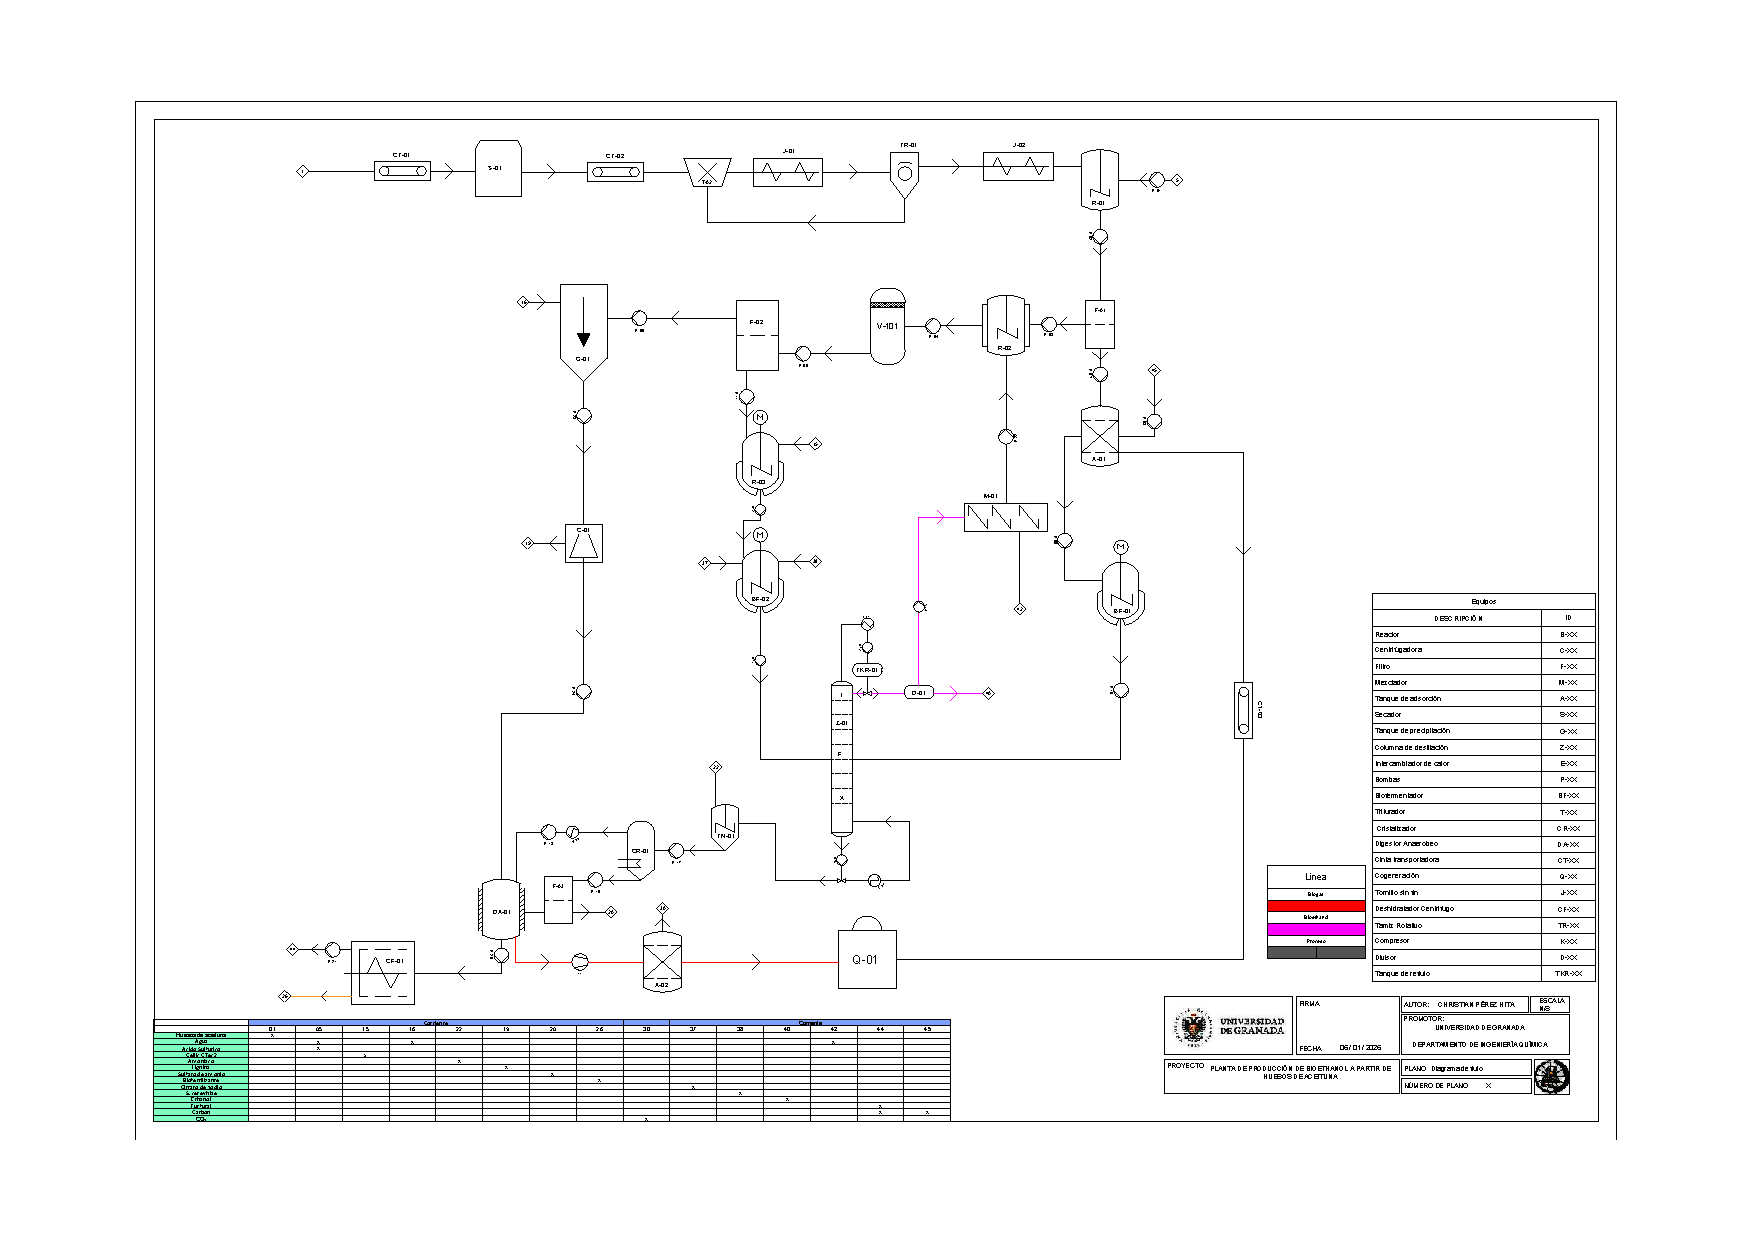
\includegraphics[width=\paperheight]{Fotos/D-flujo.pdf}%
    }
    \caption{Diagrama de flujo del proceso, fuente: elaboración propia}
    \label{fig:proceso2}
\end{figure}
\end{landscape}  % fin de página horizontal



\chapter{}
\section{Balance de materia}

Los equipos seleccionados son los siguientes:
\begin{itemize}
    \item Destilación flash
    \item Deshidratación centrifuga
\end{itemize}
\subsection{Destilación flash}
para la destilación flash se tiene la siguiente ecuación de balance de materia:
\begin{equation}
F = V + L
\end{equation}
donde F es el flujo de alimentación, V es el flujo de vapor y L es el flujo líquido.\\
Ademas para el calculo de este se utiliza la ecuación de rachford-rice:
\begin{equation}
    \sum_{i=1}^{n} \frac{z_i (K_i - 1)}{1 + \psi (K_i - 1)} = 0
\end{equation}

Donde:
\begin{itemize}
    \item $z_i$ es la fracción molar del componente $i$ en la alimentación.
    \item $K_i$ es la constante de equilibrio ($y_i/x_i$).
    \item $\psi$ es la fracción de vaporización ($V/F$).
\end{itemize}
el equilibrio se define como:
\begin{equation}
y_i = K_i x_i
\end{equation}

\noindent Debido a la falta de datos se ha considerado unos valores hipotéticos para las constantes de equilibrio:
\begin{itemize}
    \item $K_{volatiles} = 3.0$
    \item $K_{lignina} = 0.05$
\end{itemize}
\vspace{1em}
\solve{}
sustituyendo se obtiene:
\begin{equation}
\frac{0.90\cdot(3 - 1)}{1 + 2\psi}
+
\frac{0.10\cdot(0.05 - 1)}{1 - 0.95\psi}
= 0
\end{equation}

\nt{El resultado es $\psi = 0.897$}
\newpage
\subsubsection{Caudales de salida}

Para una alimentación $F = 100\ \text{kmol h}^{-1}$:

\begin{equation}
V = \psi F = 89.7\ \text{kmol h}^{-1}
\end{equation}

\begin{equation}
L = (1 - \psi)F = 10.3\ \text{kmol h}^{-1}
\end{equation}

\subsubsection{Composición de las fases}

La composición de la fase líquida se calcula como:

\begin{equation}
x_i = \frac{z_i}{1 + \psi (K_i - 1)}
\end{equation}

\begin{align}
x_1 &= \frac{0.90}{1 + 0.897\cdot(3 - 1)} = 0.322 \\
x_2 &= \frac{0.10}{1 + 0.897\cdot(0.05 - 1)} = 0.676
\end{align}

La composición de la fase vapor se obtiene de:

\begin{equation}
y_i = K_i x_i
\end{equation}

\begin{align}
y_1 &= 3.0 \cdot 0.322 = 0.966 \\
y_2 &= 0.05 \cdot 0.676 = 0.034
\end{align}
\subsection{Deshidratación Centrifuga}
Para la deshidratación centrifuga se utiliza la siguiente ecuación de balance de materia:
\subsubsection{Definición del sistema}

La corriente de alimentación $F$ (sólido húmedo) se separa en:
\begin{itemize}
    \item Una corriente de sólido deshidratado $S$
    \item Una corriente líquida separada $L$
\end{itemize}

\begin{equation}
F = S + L
\end{equation}



\subsubsection{Composición de la alimentación}

La alimentación presenta una humedad del 70\% en base húmeda:

\begin{equation}
x_{l,F} = 0.70 \qquad x_{s,F} = 0.30
\end{equation}

donde $x_{l}$ representa la fracción másica de líquido (agua) y
$x_{s}$ la fracción másica de sólido seco.



\subsubsection{Condición del sólido a la salida}

La centrífuga de alta eficiencia reduce la humedad del sólido hasta un
22\% en base húmeda:

\begin{equation}
x_{l,S} = 0.22 \qquad x_{s,S} = 0.78
\end{equation}



\subsubsection{Balance de materia del sólido seco}

Se asume que el sólido seco no se pierde con la corriente líquida:

\begin{equation}
F \, x_{s,F} = S \, x_{s,S}
\end{equation}

\noindent Para una alimentación de $F = 1000\ \text{kg h}^{-1}$:

\begin{equation}
1000 \times 0.30 = S \times 0.78
\end{equation}

\begin{equation}
S = 384.6\ \text{kg h}^{-1}
\end{equation}



\subsubsection{Balance total de materia}

\begin{equation}
L = F - S
\end{equation}

\begin{equation}
L = 1000 - 384.6 = 615.4\ \text{kg h}^{-1}
\end{equation}



\subsubsection{Comprobación del balance de líquido}

Entrada de líquido:
\begin{equation}
1000 \times 0.70 = 700\ \text{kg h}^{-1}
\end{equation}

Líquido retenido en el sólido:
\begin{equation}
384.6 \times 0.22 = 84.6\ \text{kg h}^{-1}
\end{equation}

Líquido separado:
\begin{equation}
700 - 84.6 = 615.4\ \text{kg h}^{-1}
\end{equation}

El balance de materia queda correctamente cerrado.



\subsubsection{Resultados}

\begin{itemize}
    \item Caudal de sólido deshidratado: $384.6\ \text{kg h}^{-1}$
    \item Humedad final del sólido: $22\%$
    \item Caudal de líquido separado: $615.4\ \text{kg h}^{-1}$
\end{itemize}
\nt{Estos cálculos han sido todo hipotéticos, aunque la humedad en la entrada se ha asumido las del artículo.}
\section{Uso de IA}
Para la realización de este trabajo se ha utilizado ChatGPT-4 para la corrección gramatical y ortográfica del mismo, ademas de para correciones en el codigo LaTeX mediante Github Copilot.
\printbibliography[heading=bibintoc, title={Bibliografía}]

%%\includeonly{backmatter/bibliografia} haciendolo en un capitulo aparte 
\end{document}